\documentclass[12pt,oneside,a4paper]{article}

\usepackage[backend=biber,style=numeric, sorting=none]{biblatex}
\usepackage{xcolor}
\usepackage{todonotes}
\usepackage{amsmath}
\usepackage{multicol}
\usepackage{caption}
\usepackage{hyperref}
\usepackage{graphicx}
\usepackage{listings}
\lstset{
	frame=top,frame=bottom,
	language=C,
	basicstyle=\small\normalfont,
	xleftmargin=\parindent,
	keywordstyle=\color{green!40!black},
	%  commentstyle=\itshape\color{purple!40!black},
	%  identifierstyle=\color{blue},
	%  stringstyle=\color{orange},
	morekeywords={in, globaldata, procedure, input, output, behavior, end, XOR, NOT, AND}, % keyword to highlight
	%  captionpos=t,
	tabsize=2,
	numbers=left,
	stepnumber=1,                   % the step between two line-numbers.        
	numbersep=5pt,
	framexleftmargin=10pt,
	title=\lstname,
	captionpos=t,
	showspaces=false,
}
\DeclareCaptionFormat{listing}{\rule{\dimexpr\textwidth\relax}{0.4pt}\par\vskip1pt#1#2#3}
\captionsetup[lstlisting]{format=listing,singlelinecheck=false, margin=0pt,labelsep=space,labelfont=bf}

\usepackage{booktabs}
\usepackage[noabbrev,capitalise]{cleveref}
\crefname{listing}{algorithm}{algorithms}
\Crefname{listing}{Algorithm}{Algorithms}
\renewcommand\lstlistingname{Algorithm}
\def\lstlistingcrefname{Algorithm}
\usepackage{url}

\addbibresource{biblio.bib}

\title{\textbf{RISC-V processors with Bluespec}}

\author{High Performance Processors and System\\ A.Y. 2020/2021\\\\\\\\\textbf{Riccardo Nannini}\\\\\\}

\date{\parbox{\linewidth}{\centering%
		\today\endgraf\bigskip\bigskip\bigskip\bigskip\bigskip
		Tutors: Emanuele Del Sozzo, \endgraf\medskip
		Davide Conficconi \endgraf\bigskip\bigskip
		Professor: Marco Domenico Santambrogio 
		}}
\begin{document}

\begin{titlepage}
	\centering
	\clearpage
	\maketitle
	\thispagestyle{empty}
	\vspace*{1cm}
	\vfill
	\centering
	
\includegraphics{logo_polimi.png}
\includegraphics{logo_NECST.png}
\end{titlepage}

\tableofcontents
\newpage

\begin{abstract}
Bluespec System Verilog (\textbf{BSV}) is a state-of-the-art Hardware Description Language.
Bluespec compilation toolchain (\textbf{BSC}) has been recently released as open source \cite{bsc}. The goal of the project was investigating the potentiality of said toolchain implementing different \textbf{RISC-V} processors of increasing complexity.\\
\end{abstract}

\section{Introduction} \label{sec:intro}

This report covers chronologically the path that I have followed during the development of this project.
 
It starts from a quick overview on the \textit{RISC-V} ISA, focused on the key ingredients that make this ISA one of the most trend topics in Computer Engineering.

It proceeds with the analysis of the \textit{Bluespec System Verilog} language, outlining its novelties with respect to other hardware description languages, as well as its main features and capabilities. 

The last section is devoted to the development of various RISC-V processor designs, describing in details the characteristics of each processor and motivating the various design choices, starting from a one cycle non pipelined processor and ending with a 6 stage pipelined one enriched with multiple branch predictors.

Everything I have produced within this project (code, scripts, this report itself) is available on GitHub \url{https://github.com/riccardo-nannini/BSV_RISC-V}


\section{RISC-V} \label{sec:risc-v}
\subsection{What is RISC-V}
Since the processor designs will be based on RISC-V, knowing this ISA is fundamental.

RISC-V was born in 2010 at UC Berkley by the work of graduate students Andrew Waterman, Yunsup Lee and professors David Patterson, Krste Asanovic \cite{risc-v_original}, built on the experience gained from the 4 previous major RISC ISA design from UC Berkeley (thus justifying the ‘V’).

For the scope of the project, the focus was put on the User-Level (or Unprivileged) section of the ISA.

As the name suggests, RISC-V belongs to the family of \textbf{RISC} ISAs. In particular, RISC instruction sets are characterized by \textit{small} and \textit{highly optimized} instructions that ease \textit{pipeline} implementation, along with a large number of \textit{general purpose registers}. 

RISC-V, like many other RISC ISAs, is a \textbf{load-store architecture}; this means that, apart from some exceptions, arithmetic and logic instructions operate on register and not on memory directly. Load and store instructions take care of the transit of data from memory to register and vice versa.
\subsection{Instructions set goals}
When the first paper that declared the birth of RISC-V \cite{risc-v_original} was released back in 2011, the authors stated some of the goals that they wanted to achieve when designing this instructions set. In particular the main objectives include, but are not limited to:
\begin{itemize}
	\item Provide a \textit{realistic} but \textit{open} ISA, suitable for direct hardware implementation
	\item Provide a \textbf{small} but \textbf{complete} ISA, that avoids "\textit{over-architecting}" for a particular microarchitecture style or implementation technology.
	\item Support highly-parallel multicore implementations, including heterogeneous multiprocessors
	\item Support an efficient dense \textit{instruction encoding} with variable-length instructions (generally typical of CISC ISAs).
	\item \textbf{base-plus-extension}: provide a set of standard but optional extensions.
	\item Be fully \textit{virtualizable}.
	\item Be simple to subset for educational purpose or to reduce complexity in new implementations.
\end{itemize}
In order to achieve these goals many design choices were taken, sometimes in line with other similar ISAs, sometimes with unusual decisions.

\subsection{Main features}
RISC-V has 2 base variants, \textbf{RV32} and \textbf{RV64}, providing 32-bit or 64-bit user-level address spaces respectively. A 128-bit extension is available but mostly aimed at the future of warehouse scale computing.
\subsubsection{Registers}
RISC-V uses 31 general-purpose registers  {\fontfamily{cmtt}\selectfont{x1-x31}} with  {\fontfamily{cmtt}\selectfont{x0}} hardwired to the costant 0. Moreover, 32 64-bit registers {\fontfamily{cmtt}\selectfont{f0-f31}} holding single or double-precision floating-point values are available as shown in \cref{riscv:registers}.

\begin{figure}[h]
	\centering
	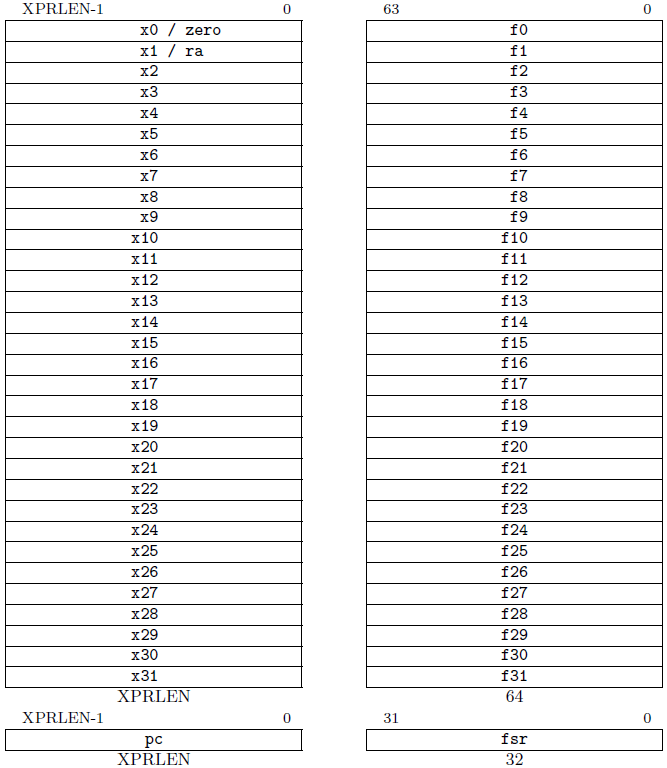
\includegraphics[scale=0.8]{risc-v_registers}
	\caption{RISC-V user-level registers (XPRLEN refers to the width of registers in bit (either 32 or 64)}
	\label{riscv:registers}
\end{figure}

There are also two special registers: the \textit{program counter} {\fontfamily{cmtt}\selectfont{pc}} holds the address of the current instruction while the \textit{floating point status register} {\fontfamily{cmtt}\selectfont{fsr}} contains the operating mode and exception status of the floating-point unit.
\subsubsection{Instruction encoding}
In addition to standard fixed-length 32-bit instructions, RISC-V supports extensions with \textbf{variable-length} ones too, useful in reducing code size specially for specific domains like embedded systems.

\cref{riscv:encoding} shows the instruction length encoding convention. 32-bit instructions have the 2 least significant bits always set to {\fontfamily{cmtt}\selectfont{1}} while the 16-bit ones must have said bits in any combination but {\fontfamily{cmtt}\selectfont{11}}.
Instructions longer than 32-bits have additional lower bits set to {\fontfamily{cmtt}\selectfont{1}}.\medskip

\begin{figure}[h]
	\centering
	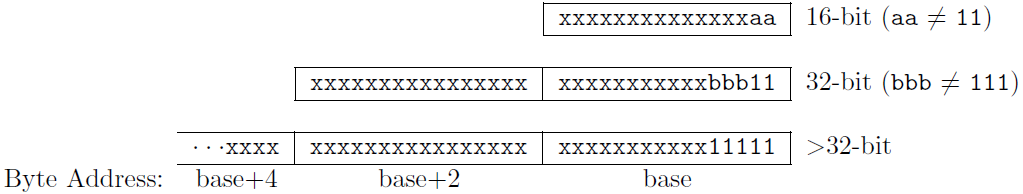
\includegraphics[scale=0.65]{risc-v_encoding}
	\caption{RISC-V instruction encoding}
	\label{riscv:encoding}
\end{figure}

\subsubsection{Instruction format}
Six basic instruction formats are present in the base version of the ISA as shown in \cref{riscv:format}.

\begin{figure}[h]
	\centering
	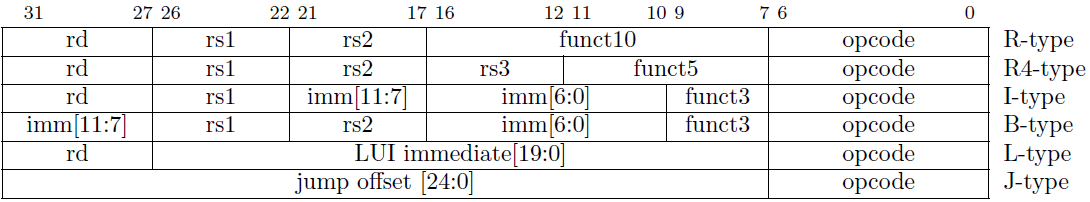
\includegraphics[scale=0.65]{risc-v_format}
	\caption{RISC-V instruction formats}
	\label{riscv:format}
\end{figure}

It is worth noting a particular design choice made by the authors. Since, as they state, the \textit{decoding} of register specifiers is usually on the \textbf{critical path} in implementations, they decided to keep all register specifiers in the same position across every instruction type. This comes with the tradeoff of having some instructions with an immediate value that has to be split in two parts.

\textbf{R-Type} instructions are for operations with two source registers (\textit{rs1} and \textit{rs2}) while \textbf{R4-Type} format is for special three source register floating point instructions. Moreover, \textbf{I-Type} format is for operations between a source register (\textit{rs1}) and an 12-bit sign-extended immediate, while \textbf{B-Type} instructions are designed for conditional branches (where the branch type is specified in \textit{funct3}).
The LUI (\textit{Load upper immediate}) operation, generally used to build 32-bit constants, is the typical instruction specified by the \textbf{L-Type}, meanwhile \textbf{J-Type} instructions encode a 25-bit target address as a PC-relative offset.

Describing in details the specification of every instruction is way out of the focus of this report and is already done with great details in the original paper \cite{risc-v_original}.\\

In the end, just a mention to the \textit{fsr}, a special register containing the status of floating-point operation, shown in \cref{riscv:fsr}.

\begin{figure}[h]
	\centering
	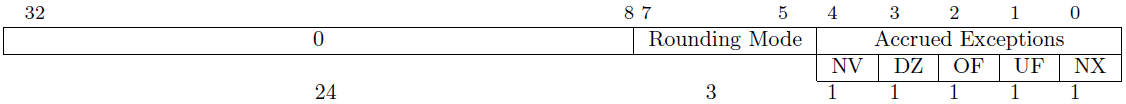
\includegraphics[scale=0.575]{risc-v_fsr}
	\caption{Floating-point status register}
	\label{riscv:fsr}
\end{figure}

It makes possible to specify the rounding mode with a specific encoding as well as reading the status of the previous floating-point operation in the flag bits.
\subsection{License}
Until here the main features of RISC-V were summarized.
Despite being a really well designed standard, this by itself does not explain the popularity of this ISA.

In fact, one of the main factor of his success is that RISC-V is provided under a \textbf{free open source} license that does not require fees to use.

This is quite unusual in the instruction set architectures world, that for a great majority are \textit{proprietary} due to historical or business reasons. Companies like ARM, IBM and Intel have patents on their ISAs which prevent others from using them without licenses.

Negotiations for said licenses can take 6-24 months and can cost up to \$1M-\$10M, ruling out academia and other with small volumes. An ARM license, for instance, doesn't even let you design an ARM core; you just get to you \textit{their} designs \cite{risc-v_free}.

Some open-source ISA already existed but were not as popular and well designed as RISC-V is.\\

The birth of this standard enabled a \textbf{real free open market} of processor designs leading to:
\begin{itemize}
	\item greater innovation via \textbf{free-market competition}
	\item shared open core designs
	\item processors becoming \textbf{affordable} for more devices
\end{itemize}

\section{BSV}
\section{Processor designs}
\newpage
\printbibliography

\end{document}


